
\exercice{Shapes --  Part I}

We would like to write a program allowing us to create some simple geometric
shapes. The program should allow us to draw the shapes, show the list of all
shapes, compute the sum of areas and the sum of circumference of all
geometric shapes.

A typical use-case was shown during the lecture and the sample code is provided
online~\cite{WEBGL} (file Shapes\_Solution.jar).

After important this program into your IDE you will find the following
additional functionality:
\begin{itemize}
 \item Each geometric shape has a unique ID.
 \item Upon showing the list of created shapes, the ID is shown together with
other information for each shape.
\item The user can modify some of the properties of each shape (size etc.).
\item The user can delete all existing shapes.
\end{itemize}

The geometric shapes have to be implemented following the hierarchy given in
Figure~\ref{Inherit} on page~\pageref{Inherit}


%\renewcommand{\figurename}{Figure}
\begin{figure}[htb]
  \begin{center}
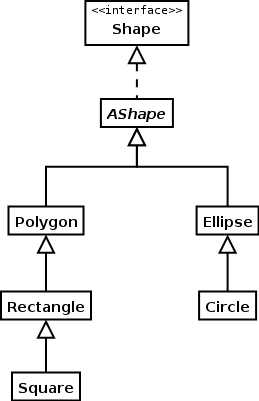
\includegraphics[height=7cm]{\compilationpath/Exercices/ex3/latex/resources/figures/inherit.png}
    \caption{Hierarchy of geometric shapes}
    \label{Inherit}
  \end{center}
\end{figure}

The \texttt{Shape} interface contains the following methods:
\begin{itemize}
 \item \texttt{double perimeter()}: return the circumference of a shape.
 \item \texttt{double area()}: return the area of a shape.
 \item \texttt{void change()}: allows the modification of a shape.
 \item \texttt{int getID()}: returns the unique ID of a shape.
 \item \texttt{void setID()}: fixes the unique ID of a shape.
 \item \texttt{String toString()}: prints a shape as ASCII text.
 \item \texttt{void draw(Graphics g)}: prints a shape on the screen.
 \item \texttt{boolean contains(Point p)}: test if a given point \texttt{p} is
inside a given shape or not.
\end{itemize}

Some explanations regarding the implementation of the shapes application:
\begin{itemize}
 \item The perimeter \texttt{P} of an ellipse can be approximated by a formula
discovered by the indian mathematician \emph{Srinivasa Aiyangar Ramanujan
(1887-1920)} in 1914:$$P\approx\pi\cdot\sqrt{\frac{2(a^2+b^2)-(a-b)^2}{2}}$$
where $a$ and $b$ are the small and the big diameter respectively.
\item The area $A$ of a polygon can be computed by the following forumula (based
on Green's Theorem in the plane):
$$A=\frac{1}{2}\sum_{i=0}^{n-1}a_i \text{ avec } a_i=x_iy_{i+1}-x_{i+1}y_i$$
where the points $(x_i, y_i), i=0,\ldots ,n$ with $x_0=x_n$ and $y_0=y_n$ are
the points constructing the polygon. \textbf{Remark:} this formula gives an
erronous value if the poglygon is not convex.
\item A point $P$ $(p_1,p_2)$ is inside a circle $C$ with center $(x_1, x_2)$ and diameter $r$ if
$$(p_1 - x_1)^2 + (p_2-x_2)^2 \leqslant r^2$$
\item A point $P$ $(p_1, p_2)$ is inside an ellipse $\mathcal{E}$ with width $w$,height $h$ and center $(x_1, x_2)$ if $$\left(\frac{p_1 - x_1}{w}\right)^2 + \left(\frac{p_2-x_2}{h}\right)^2 \leqslant 1$$
\item The mathematical function \texttt{sqrt(x)} is found in the \texttt{java.lang.Math} package (see~\cite{JAVAAPI}).
\item The class \texttt{java.awt.Graphics} allows you to draw geometric shapes (see~\cite{JAVAAPI}).
\item You will find online~\cite{WEBGL} a skeleton of the implementation. The code has gaps you have to fill. They are indicated by the following comment: \texttt{Add your code for the Serie 2(1) of Genie Logiciel here!!}.
\item All the necessary classes are in the distributed zip file:
\begin{itemize}
 \item Complete the \texttt{Polygon.java} and the \texttt{WorkShapes.java} files.
 \item Create the files \texttt{Ellipse.java} and \texttt{Circle.java} accordingly to the above discussion.
\end{itemize}
\item The class \texttt{WorkShapes} is the main class of the application. It implements most parts of the GUI. Fill the gaps indicated by the comment:
\texttt{Add your code for the Serie 2(1) of Genie Logiciel here!!}.
\item Starting with the distributed files, create a new project in your IDE and edit the code and the GUI as discussed.
\item Check that your code is working by playing around with the new application.
\item Edit the dialog box \texttt{shapes.gui.About.java} and put your names in here.
\item The application can be launched the following ways:
\begin{itemize}
 \item From console: \texttt{java shapes.WorkShapes}
 \item From ANT: \texttt{ant run}
 \item From your IDE
\end{itemize}


\end{itemize}

\exercice{Shapes -- Part 2}

Starting from Part 1, implement the following extensions:
\begin{itemize}
 \item The application should also handle triangles. Thus, create the class \texttt{Triangle.java} exending \texttt{Polygon.java}. Remember that the area of a triangle can be computed with the following formula: $$A=\sqrt{p(p-a)(p-b)(p-c)} \text{ avec } p=\frac{a+b+c}{2}$$
 \item Implement a function allowing to sort the list of shapes in ascending order:
 \begin{itemize}
  \item by area
  \item by perimeter
  \item by ID
 \end{itemize}
 These operations refer to the menu entries \emph{Sort by Area}, \emph{Sort by Perimeter} and \emph{Sort by ID} of the \emph{Edit} menu.
\item It should be possible to move either one particular shape or all shapes togheter. These operations refer to the menu entries \emph{Move} and \emph{Move all} of the \emph{Edit} menu.
\item It should be possible to delete a given shape. This operation refers to the menu entry \emph{Delte a shape} of the \emph{Edit} menu.
\item It should be possible to save a list of shapes to the harddrive. Moreover, it should also be possible to open such a file and show all the shapes as defined in the file. These operations refer to the menu entries \emph{Open} and \emph{Save as...}
\end{itemize}

Some indications:
\begin{itemize}
 \item The solution of Part 1 is available online~\cite{WEBGL}: \texttt{Shapes\_Solution.jar}. Download this archive and get familiar with the application.
 \item The application can be started with: \texttt{java -jar Shapes\_Solution.jar}
 \item To sort the list of shapes, use the \texttt{java.util.Collections} class and its static method \texttt{sort(List \_list, Comparator \_c)}
 \item You have to implement the following comparators by extending the \texttt{java.util.Comparator} interface:
 \begin{itemize}
  \item \texttt{ByAreaShapesComparator},
  \item \texttt{ByPerimeterShapesComparator} and
  \item \texttt{ByIDShapesComparator}.
 \end{itemize}
  See~\cite{WEBGL} for additional information.
  \item In order to be able to save the list of shapes to the harddrive, all shapes have to implement the \texttt{java.io.Serializable} interface (see~\cite{JAVAAPI}). Therefore, it is recommended to modify the \texttt{Shape} class like: \\ \verb"        public interface Shape extends java.io.Serializable"\\
  \item To learn how to write objects into files and read them back from files, have a look at the documentation of the \texttt{java.io.ObjectOutputStream} and \texttt{java.io.ObjectInputStream} classes. (see~\cite{WEBGL}).
  \item Rember that after loading a list of shapes from the harddrive new shapes can be added to the list (Hint: ID).
  \item Don't spend too much time about handling special cases when saving/reading files (like erase already existing file etc.). A short error message is enough.
  \item Take as starting point the source code provided online~\cite{WEBGL} (\texttt{donnee\_s1\_e1.zip}) and fill the gaps indicated by the comments:
  \begin{itemize}
   \item \texttt{Add your code for the Serie 1(1) of Genie Logiciel here!!}
   \item \texttt{Add your code for the Serie 1(2) of Genie Logiciel here!!}
   \item In Netbeans open the \texttt{Action Items} (Windows -> Action Items).
  \end{itemize}

\end{itemize}


